\section{实验原理}
\subsection{总体框架及通路图}
\begin{figure}[htbp]
    \centering
    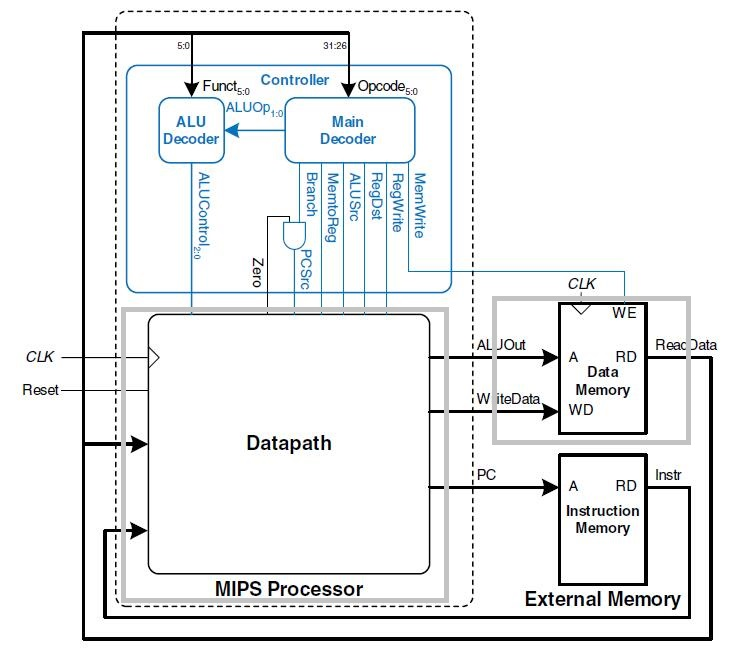
\includegraphics[width = 0.7\textwidth]{image/mips_framework.png}
    \caption{单周期CPU框架图}
    \label{fig:mips_framework}
\end{figure}
如图~\ref{fig:mips_framework},完整的单周期CPU实现框架图。其中灰色线框外的部分已在实验二中完成,继续完成datapath,即可将单周期MIPS软核完整实现。

\begin{figure}[htbp]
    \centering
    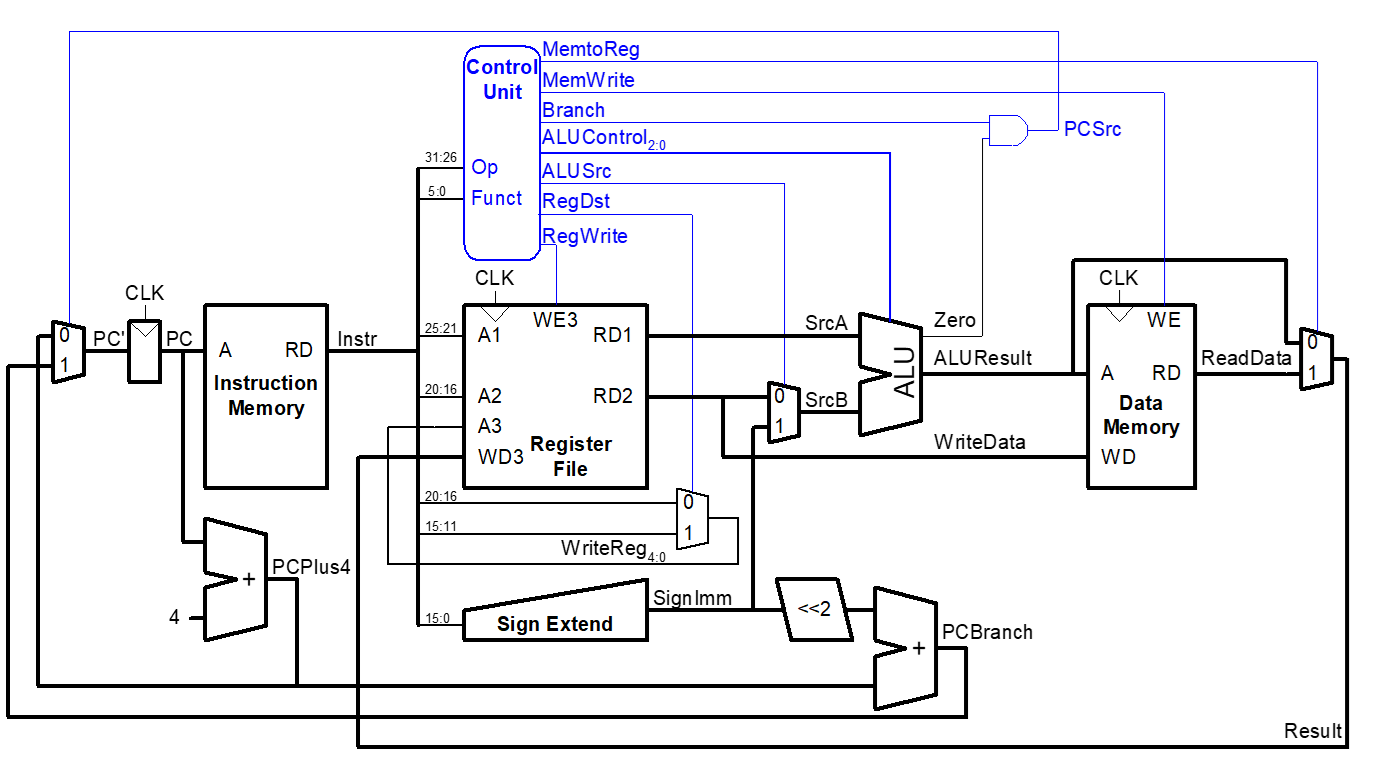
\includegraphics[width = 0.8\textwidth]{image/mips_single_cycle_datapath.png}
    \caption{单周期CPU框架图}
    \label{fig:mips_single_cycle_datapath}
\end{figure}

图~\ref{fig:mips_single_cycle_datapath}为单周期的完整通路图,涵盖\textit{add、and、sub、or、slt、beq、j、lw、sw、addi}等指令。实验三仅实现上述指令,完整的MIPS指令集将与硬件综合设计中完善,此处以掌握数据通路分析为主要目的。

\subsection{控制器译码信号规范}
% 数据通路连接前,
\subsubsection{ALU控制码译码}
由于控制器的设计在实验二中并不进行强制限制,因此ALUOp信号在部分设计中可能不会存在,只需按照表~\ref{tab:alu_decoder}中其他信号即可
\begin{table}[htbp]
    \centering
    \begin{tabular}{l|l|l}
        \hline
        ALUOp[1:0]&	Funct&	        ALUControl[2:0]\\ \hline
        00&	        X(for lw)&	            010 (Add) \\
        01&	        X(for beq)&	            110 (Subtract) \\
        10&	        100000 (add)&	010 (Add) \\
        10&	        100010 (sub)&	110 (Subtract)\\
        10&	        100100 (and)&	000 (And) \\
        10&	        100101 (or)&	001 (Or) \\
        10&	        101010 (slt)&	111 (SLT)\\ \hline
 
    \end{tabular}
    \caption{ALU控制码译码信号表}
    \label{tab:alu_decoder}
\end{table}

\textcolor{red}{这里需要注意,不按照表中的信号也可,只要保证不同运算的alucontrol信号不同即可。}
\subsubsection{信号控制码译码信号}
信号控制码译码信号与实验二相同,在通路连接时分别接入到需要控制的端口。
\begin{table}[htbp]
    \centering
    \begin{tabular}{l|l|l|l|l|l|l|l|l}
         instruction&	op[5:0]&	regwrite&	regdst&	alusrc&	branch&	memWrite&	memtoReg&	aluop[1:0]\\ \hline
        R-type&	000000&	1&	1&	0&	0&	0&	0&	10\\
        lw&	100011&	1&	0&	1&	0&	0&	1&	00\\
        sw&	101011&	0&	X&	1&	0&	1&	X&	00\\
        beq&	000100&	0&	X&	0&	1&	0&	X&	01\\
        addi&	001000&	1&	0&	1&	0&	0&	0&	00\\
        j&	000010&	0&	X&	X&	X&	0&	X&	XX \\ \hline
 
    \end{tabular}
    \caption{控制信号译码}
    \label{tab:controller_decode}
\end{table}

\subsection{数据通路连接}
在进行数据通路连接前,除了三大基本器件,还有些许小器件需要实现,包括加法器、触发器、多路选择器、移位器、符号扩展器件等。这些器件多为简单的组合逻辑,在数字逻辑课程已有涉及,此处不再赘述,具体实现参见附录。

\subsubsection{LW指令}
以LW指令为例构建基本的单周期CPU数据通路,需要的基本器件有PC、Regfile、存储器,见图~\ref{fig:0_MIPS_state_elements},其他小的组合逻辑部件根据需求进行添加。

\begin{figure}[htbp]
	\centering
	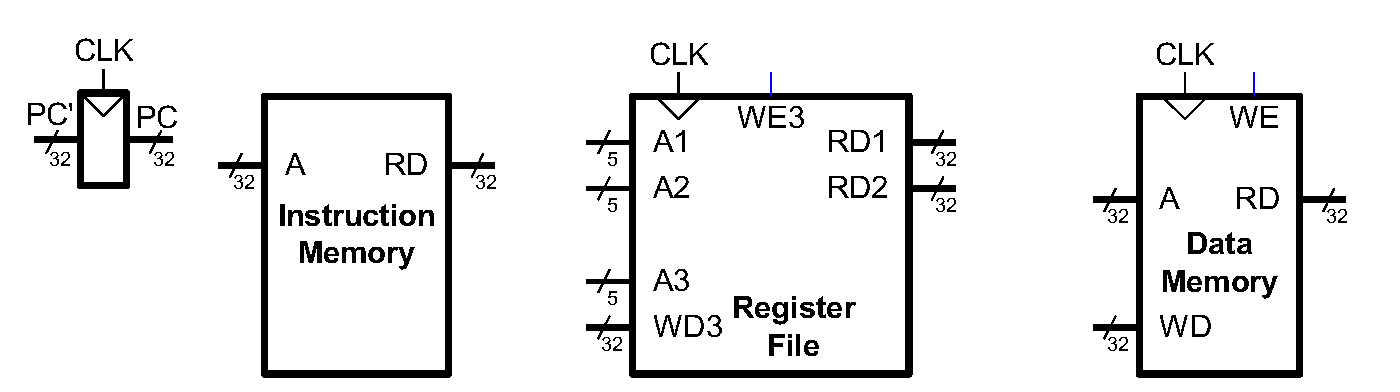
\includegraphics[width=1.0\textwidth]{image/0_MIPS_state_elements.pdf}
	\caption{\label{fig:0_MIPS_state_elements}}
\end{figure}

第一步为取值,将PC(即指令地址)输出至Instruction Memory(指令存储器)的address端口,如图~\ref{fig:1_lw_fetch}。

\begin{figure}[htbp] 
	\centering
	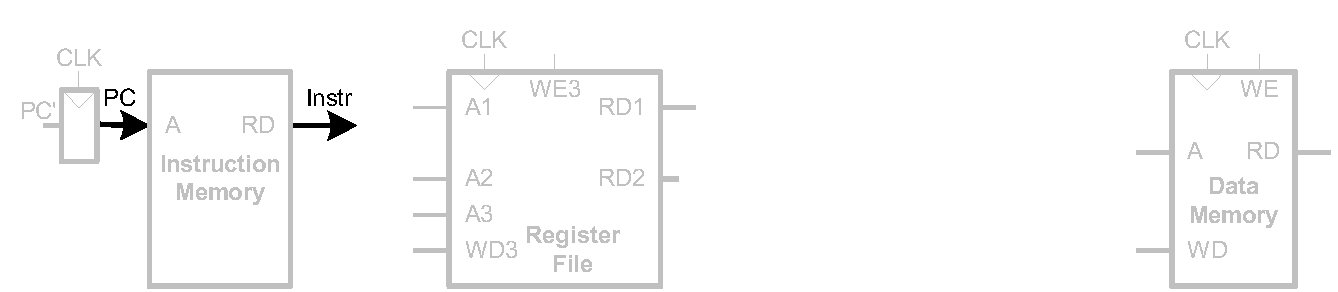
\includegraphics[width=1.0\textwidth]{image/1_lw_fetch.pdf}
	\caption{\label{fig:1_lw_fetch}}
\end{figure}

LW指令的汇编格式为:LW rt,offset(base),其中base(基地址)为指令[25:21]所指向的寄存器值,offset(地址偏移)为指令[15:0]。将 base 寄存器的值加上符号扩展后的立即数 offset 得到访存的地址,根据地址从存储器中读取1个字(连续4个字节)的值写入到 rt 寄存器中。

根据LW指令的定义,将指令存储器读出的指令([31:0])中[25:21]连接至regfile寄存器堆的第一个输入地址,即Address1(A1)。
\begin{figure}[htbp]
	\centering
	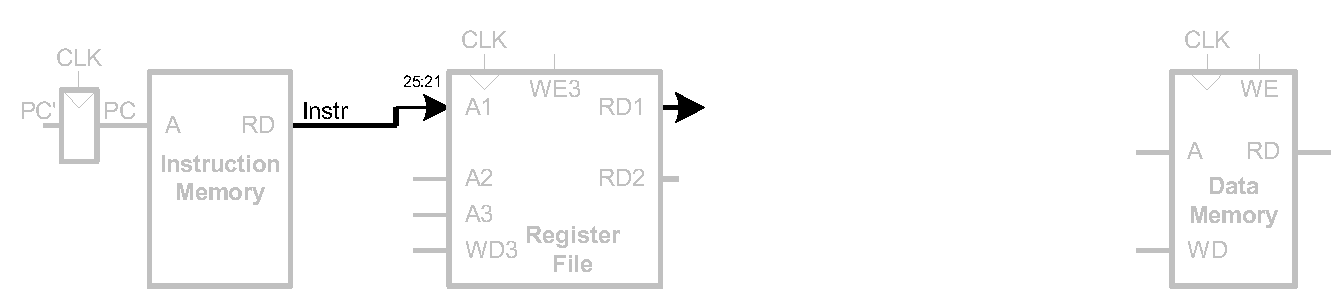
\includegraphics[width=1.0\textwidth]{image/2_lw_register_read.pdf}
	\caption{\label{fig:2_lw_register_read}}
\end{figure}

除此之外需要将offset进行扩展,因而将指令[15:0]传至\textcolor{red}{有符号}扩展模块,输出32位的符号扩展信号(SignImm)。
\begin{figure}[htbp]
	\centering
	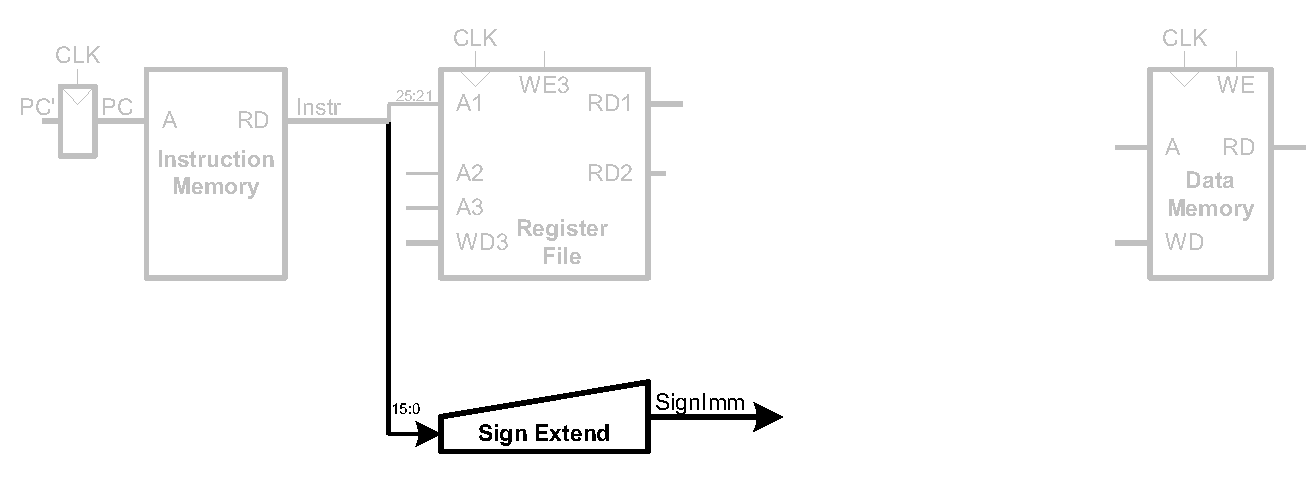
\includegraphics[width=1.0\textwidth]{image/3_lw_immediate.pdf}
	\caption{\label{fig:3_lw_immediate}}
\end{figure}

得到基地址base和offset后,需进行加法计算,其操作可以采用如下描述:Addr ← GPR[base] + sign\_extend(offset)。加法计算使用ALU中设计实现的加法运算,因而图~\ref{fig:4_lw_address}中,RD1读出的GPR[base]和经过有符号扩展后的sign\_extend(offset)分别作为ALU的两个输入(SrcA、SrcB),经过ALU进行加法运算后,得到ALUResult作为地址,输入到数据存储器Data Memory的Address端口。

这里需要注意的是,由于计算地址与进行加法运算相同,所以用于控制ALU运算类型的信号ALUControl与加法运算应该相同,如图~\ref{fig:4_lw_address}中蓝色部分所示。AlUControl信号由Controller译码得到,在此不再赘述。
\begin{figure}[htbp]
	\centering
	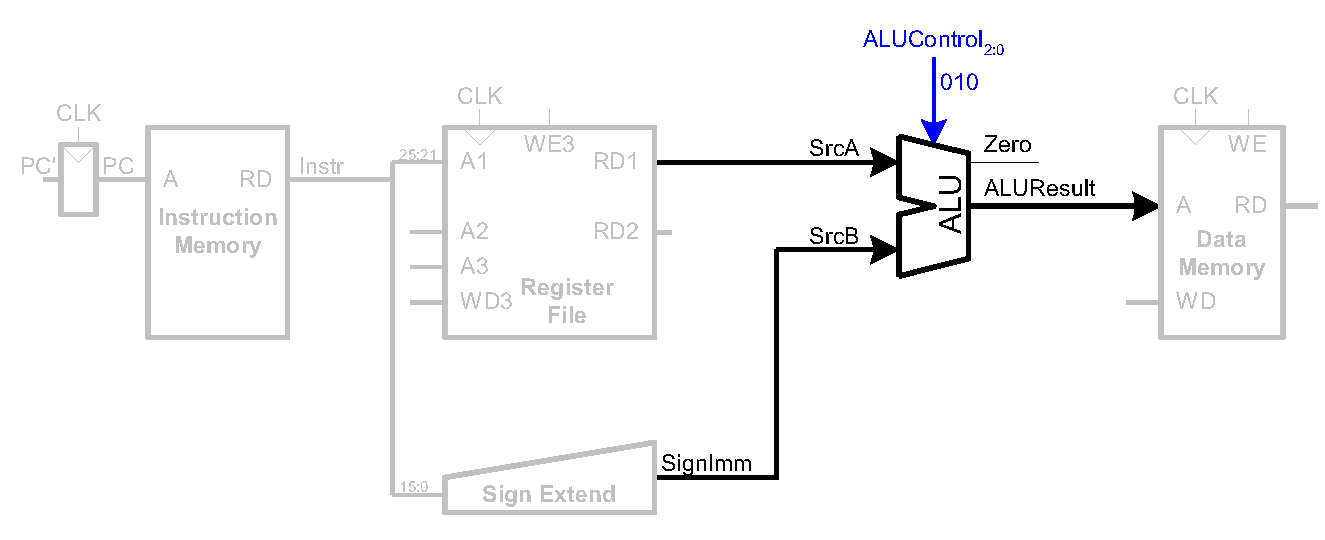
\includegraphics[width=1.0\textwidth]{image/4_lw_address.pdf}
	\caption{\label{fig:4_lw_address}}
\end{figure}

\newpage
将地址输入后,将数据存储器读出的数据写回到regfile中,其地址为rt,即指令的[20:16]。如图~\ref{fig:5_lw_memory_read},连接时需要将指令[20:16]连接至寄存器堆的Address3(A3)端口,对应的数据信号ReadData连接至WriteData3(WD3)端口。

\begin{figure}[htbp]
	\centering
	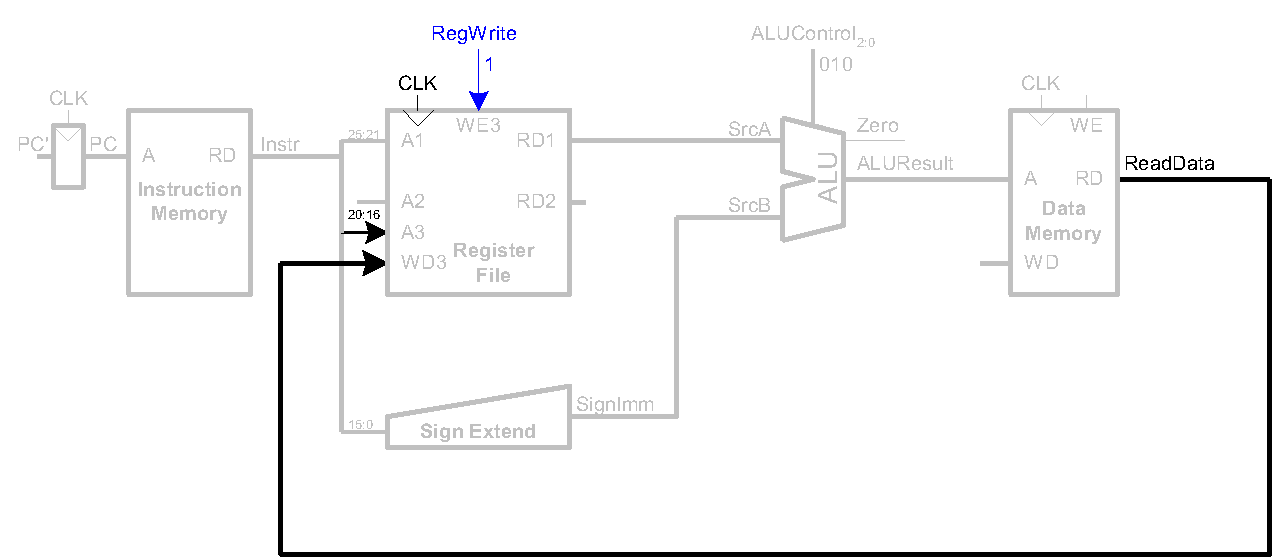
\includegraphics[width=1.0\textwidth]{image/5_lw_memory_read.pdf}
	\caption{\label{fig:5_lw_memory_read}}
\end{figure}

完成上述连接后,一条能够满足LW指令执行的数据通路即完成。LW指令执行结束后,需开始下一条指令的执行,重复同样的执行过程。唯一的不同在于PC地址需要变为下一条指令所在地址。由于实现的是32位MIPS指令集,并且采用字节读写的方式,因为需要读取后续4个字节的数据,即PC+4。将得到的PC+4信号写入PC(D触发器)的输入端,即可实现每周期地址+4的操作。

\textcolor{red}{注意:这里我们不采用很多参考书籍中复用ALU的方式计算加法,而是使用一个单独的加法器模块,如图~\ref{fig:6_lw_pc_increment},原因在于,ALU在实现多种运算逻辑后,其组合逻辑更加复杂,复用ALU进行PC+4的运算需要控制信号、输入的多路选择,增加了设计的复杂性的同时,也不符合硬件电路设计的思维。在电路设计中的复用更多是出于简化设计、优化延迟、降低功耗等目的,而非单一功能完成后进行复用的软件设计思维。}

\begin{figure}[htbp]
	\centering
	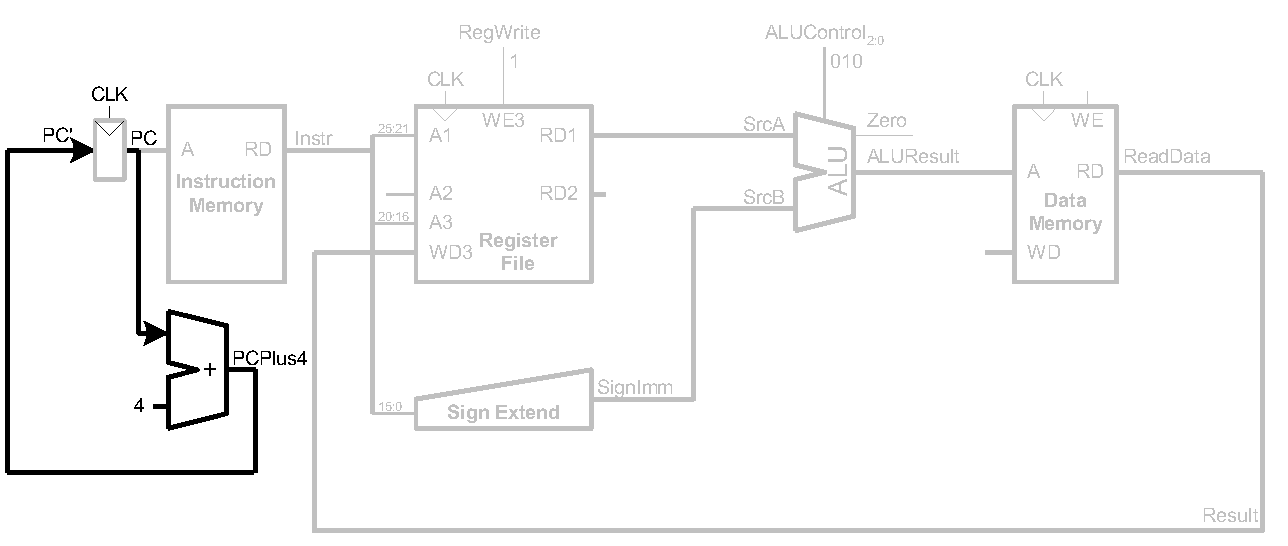
\includegraphics[width=1.0\textwidth]{image/6_lw_pc_increment.pdf}
	\caption{\label{fig:6_lw_pc_increment}}
\end{figure}

\subsubsection{SW指令}
在完成LW指令的数据通路后,SW指令仅需进行些许改动即可。首先来看SW指令的定义:SW rt,offset(base)。从指令格式和译码的数据域来看,与LW无异。其区别在于,LW需要从数据存储器读取数据并写入regfile,而SW仅需要将数据写入数据存储器。计算地址的GPR[base]+sign\_extend(offset)不变,但rt变为读取寄存器,因而需要将其连接至Address2(A2),读出的数据RD2信号连接至数据存储器的WD端口。

这里涉及到几个控制信号的值,分别为MemWrite和RegWrite,均连接至写使能端口WE,值为1时使能,为0时不使能。如图~\ref{fig:sw}所示,在进行存储器读写时,MemWrite需要使能,置1。虽然此时执行的是sw写操作,但是ReadData信号会是什么值?这取决于使用的Memory类型,假设会有随机值读出,A3(write address)同时将指令的[20:16]写入,这时将会有错误的值写到寄存器堆中。为了避免这种情况,需要将RegWrite置为0,此时无法对寄存器堆进行写操作。\textcolor{blue}{这里进行延伸,所有不对寄存器堆进行写操作的指令,都可能会有类似的情况发生,因此这种类型的指令都应该将regfile的写使能关闭。同理,所有不对指令寄存器进行读写的指令,也应当关闭其使能端口,避免意外情况的出现。}

\begin{figure}[htbp]
	\centering
	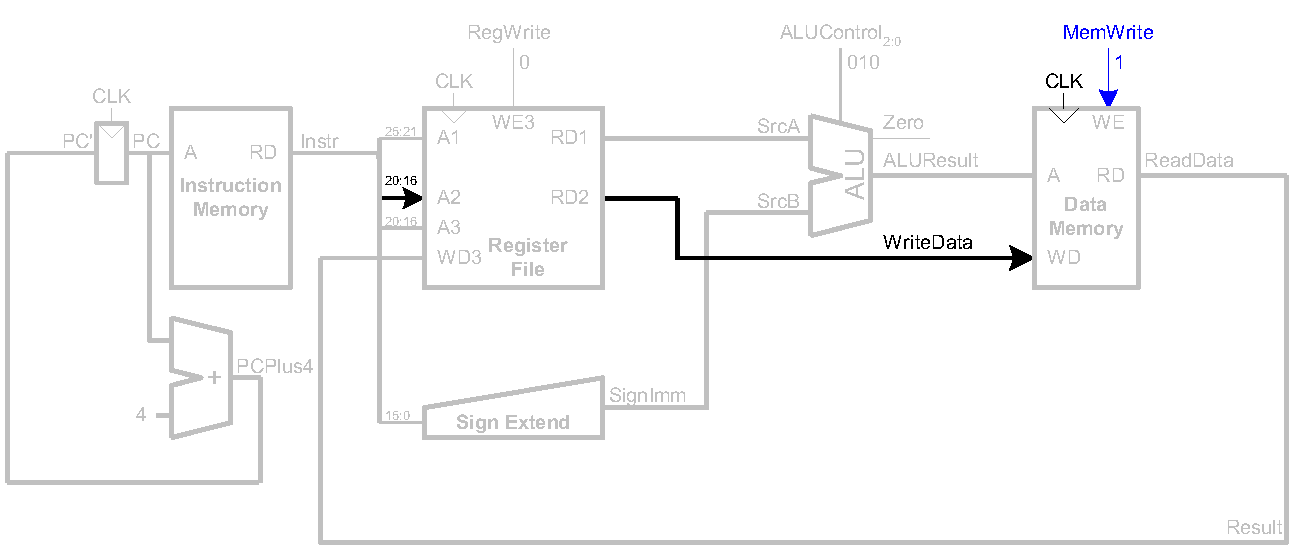
\includegraphics[width=1.0\textwidth]{image/sw.pdf}
	\caption{\label{fig:sw}}
\end{figure}
\subsubsection{R-Type指令}
R-Type是MIPS指令中一大类指令的合集,均为XXX rs,rt,rd形式的指令。除了指令进行的运算类型不同外,其操作均为将rs,rt所在寄存器的值进行相应运算后,存入rd中。因而,对已经满足lw、sw的数据通路进行一定改造即可。

通路改造方法为添加多路选择器。lw指令写入regfile的地址为rt,而R-Type为rd,在此处加入一个多路选择器,输入分别为指令的[20:16]和[15:11],使用RegDst(register destination)信号控制,多路选择其输出信号命名为WriteReg(write register)。ALU输入为rs,rt,分别对应srcA,srcB,因此需要在srcB处加入多路选择器,选择来源为RD2或立即数SignImm,控制信号为ALUSrc(ALU source)。最后写回到regfile的值应该为ALU计算得到的值,为ALUResult,加入多路选择器控制Result来源为ALU或数据存储器,控制信号为MemtoReg(Memory to regfile)。

\begin{figure}[htbp]
	\centering
	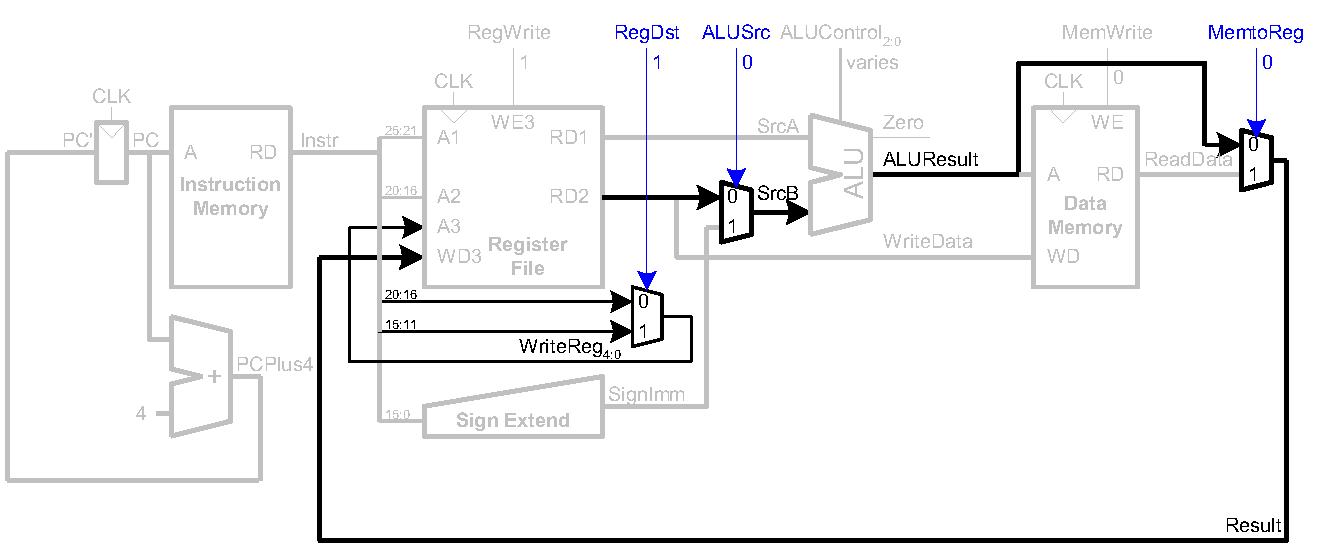
\includegraphics[width=1.0\textwidth]{image/R-type.pdf}
	\caption{\label{fig:R-type}}
\end{figure}
\subsubsection{Branch指令}
接下来添加分支指令,即通过条件判断是否需要跳转。此处以beq指令为例。其定义为:BEQ rs, rt, offset。如果寄存器 rs 的值等于寄存器 rt 的值则转移,否则顺序执行。转移目标由立即数 offset 左
移 2 位并进行有符号扩展的值加上该分支指令对应的\textcolor{blue}{延迟槽指令的 PC}计算得到。

这里暂时无须考虑延迟槽的概念,只需要知道其地址为PC+4,即当前指令的下一条指令所在的地址。
\begin{figure}[htbp]
	\centering
	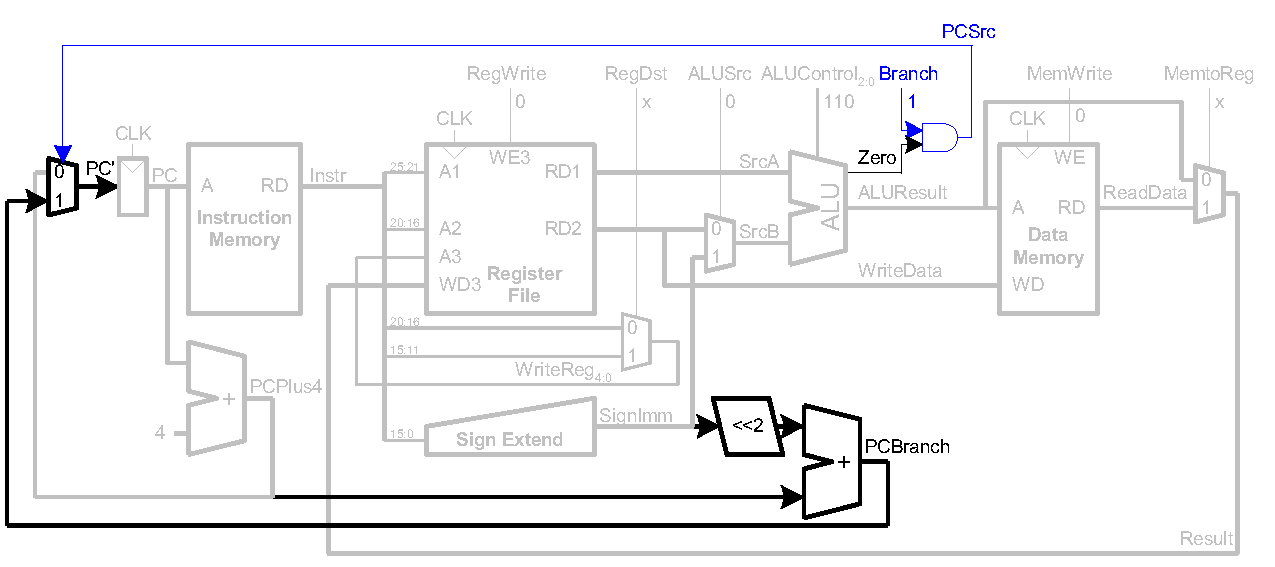
\includegraphics[width=1.0\textwidth]{image/beq.pdf}
	\caption{\label{fig:beq}}
\end{figure}

beq需要三步操作,分别为条件判断,偏移计算,PC转移,下面分别实现每步操作。条件判断需要判断rs、rt所在的寄存器值是否相等,可以使用ALU的减法进行计算,输出zero信号,并与译码得到的Branch信号(判断是否为分支指令)进行and操作,作为PCSrc信号。第二步偏移计算公式为:
\begin{itemize}
    \item target\_offsetSign\_extend(offset||$0^{2}$)
    \item PC$\leftarrow$PC + target\_offset
\end{itemize}

先将offset左移2位后,再进行有符号扩展,最后与PC+4相加。最后PC转移根据PCSrc信号进行控制,满足条件时,PCSrc为1,选择PCBranch作为下一条指令的地址。通路图修改见图~\ref{fig:beq}。


% \subsubsection{I-Type指令}

\subsubsection{J指令}
跳转指令实际为无条件跳转,不需要做任何判断,因此更加简单。只需要计算地址,更改PC即可。其跳转目标由该指令对应的延迟槽指令的 PC(PC+4)的最高 4 位与立即数 instr\_index(instr[25:0])左移 2 位后的值拼接得到。如图~\ref{fig:j},instr[25:0]左移2位,拼接pc[31:28],而后通过多路选择器。多路选择器直接由jump进行控制。
\begin{figure}[htbp]
	\centering
	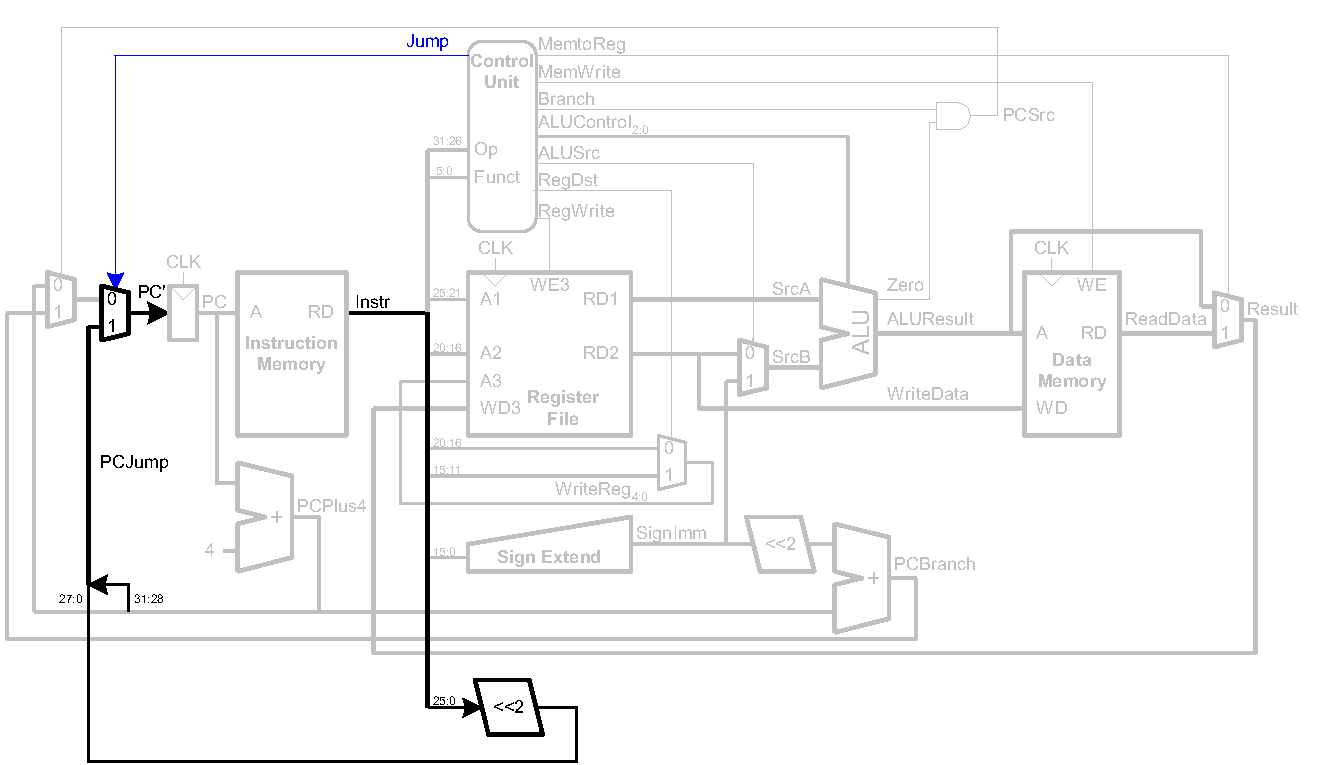
\includegraphics[width=1.0\textwidth]{image/j.pdf}
	\caption{\label{fig:j}}
\end{figure}